%%%%%%%%%%%%%%%%%%%%%%%%%%%%%%%%%%%%%%%%%%%%%%%%%%%%%%%%%%%%%%%%%%%%%%%%%%%%%%%%%%%%%%%%%%%%%%%%%%%%%%%

\documentclass[prb,aps,nofootinbib,superscriptaddress,floatfix]{revtex4-2} 
\usepackage{graphicx}
\usepackage{xcolor} 
\usepackage{amsmath}
\usepackage{amssymb} 
\usepackage{natmove}
\usepackage{natbib}
\usepackage{hyperref} 
\usepackage{bm}

%%%%%%%%%%%%%%%%%%%%%%%%%%%%%%%%%%%%%%%%%%%%%%%%%%%%%%%%%%%%%%%%%%%%%%%%%%%%%%%%%%%%%%%%%%%%%%%%%%%%%%%

\begin{document}

\title{The Mechanism of Shrimpoluminescence}

\author{Tyler C. Sterling}
\email{ty.sterling@colorado.edu}
%\affiliation{Department of Physics, University of Colorado at Boulder, Boulder, Colorado 80309, USA}

\date{\today}

\begin{abstract}
Snapping shrimp can produce bubbles that emit light when they collapse. The light emission is known as \emph{shrimpoluminescence} in the case of shrimp, but more generally when an acoustically driven bubble emits light, it is called \emph{sonoluminescence}. We would like to understand how the light is emitted. In this paper, we will specialize to the case of a single, stable bubble driven to produce light over many cycles. We will derive the bubble's equation of motion and examine the conditions in its interior. It turns out that, when the bubble collapses in a process known as \emph{cavitation}, the gas trapped in the bubble becomes hot enough to ionize. Light is emitted as black-body radiation with electron-ion bremsstrahlung, electron-atom bremsstrahlung, and electron-ion recombination limiting the amount of light that escapes the bubble.
\end{abstract}

\maketitle

\section{Introduction}
Snapping shrimp, like our cute friend in fig. \ref{fig:shrimp}, are known to produce cavitating bubbles by snapping their claws \cite{versluis2000snapping,lohse2001snapping,tang2019bioinspired}. They have a strong appendage (the \emph{dactyl}) in thier claw (fig. \ref{fig:shrimp} [center]) that is used to create a high-velocity jet of water. The low pressure region in the jet's wake forms a bubble (fig. \ref{fig:shrimp} [right]) that produces an exceptionally loud noise when it collapses. The sound produced by even one shrimp's snap is detectable over a mile away \cite{everest1948acoustical}. The noise produced by groups of shrimp is so intense that the U.S. Navy used them as ``sonar-camouflage" in the Pacific ocean during World War II \cite{versluis2000snapping}. The shrimp were not patriots helping the war-effort, however; they snapped for food. The sound wave produced by the cavitating bubble is used to stun or kill prey \cite{versluis2000snapping}. If the shrimp's prey had very\footnote{Shrimpoluminescence is too weak to be seen by the naked-eye.} sensitive eyes (and also were not dead) they might notice a flash of light is also produced through an effect referred to as ``shrimpoluminescence" in the case of the pistol shrimp \cite{lohse2001snapping}, but more generally known as \emph{sonoluminescence}.


\begin{figure}
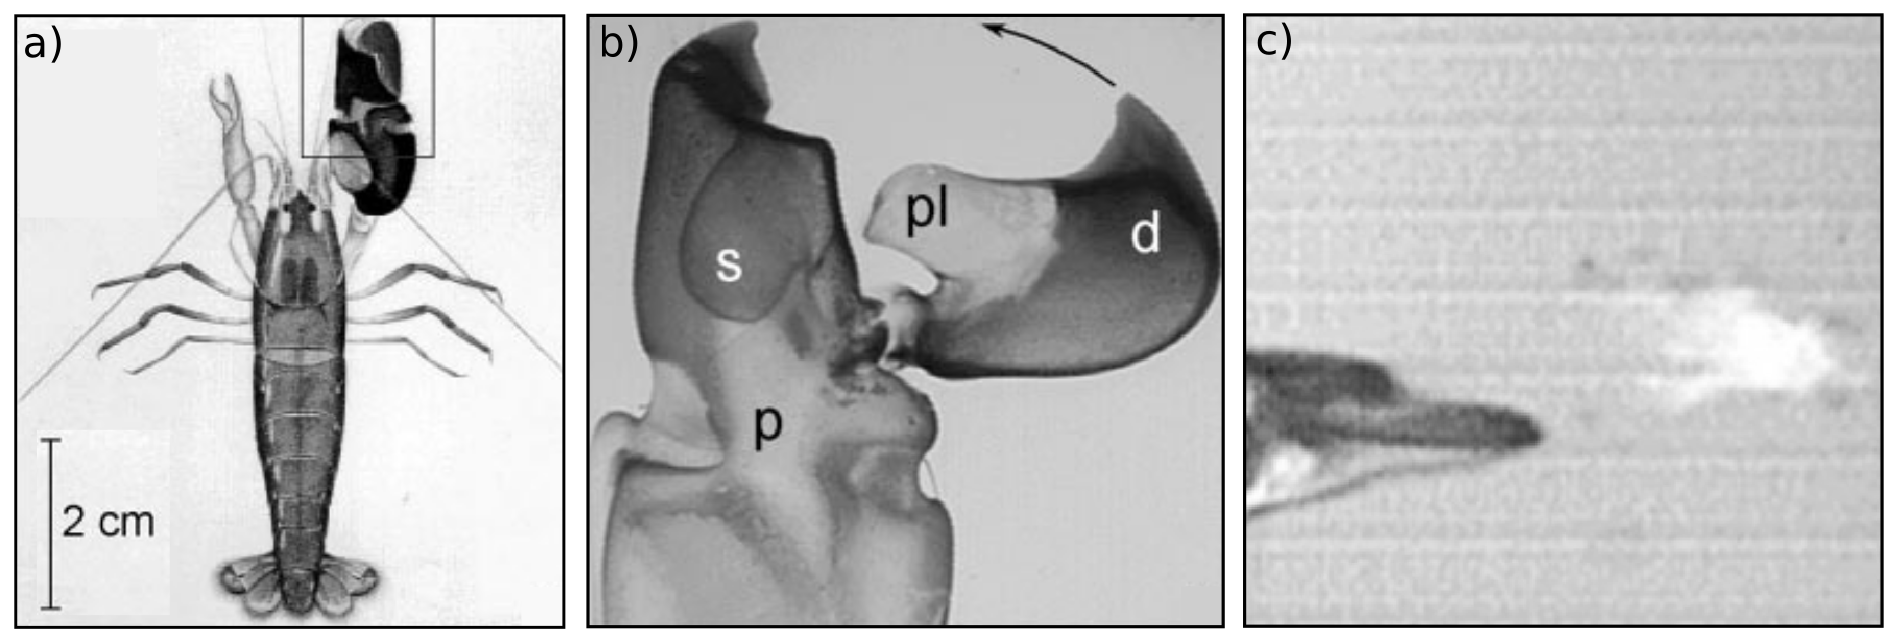
\includegraphics[width=0.95\linewidth]{figs/shrimp.pdf}
    \caption{(left) Snapping shrimp (\emph{Alpheus heterochaelis}). (center) Blown-up view of the shrimp's claw. The \emph{plunger} (pl) on the \emph{dactyl} (d) rapidly enters the \emph{socket} (s), ejecting a high-velocity jet of water. A time near the bubble collapse is shown on the right. The light emission is too dim to be seen by the naked eye. Adapted from refs. \cite{versluis2000snapping} and \cite{lohse2001snapping}.}
\label{fig:shrimp}
\end{figure}

Sonoluminescence (SL) is defined as the process by which a ``driven gas bubble collapses so strongly that the energy focusing at collapse leads to light emission" \cite{brenner2002single}. SL comes in two forms: (i) single-bubble sonoluminescence and (ii) multi-bubble sonoluminescence. Multi-bubble sonoluminescence (MBSL) consists of  ``the simultaneous creation and destruction of many separate, individual cavitation bubbles" \cite{crum1994sonoluminescence,brenner2002single}, whereas in single-bubble sonoluminescence (SBSL), rather obviously, only a single bubble is present \cite{gaitan1992sonoluminescence}. The discovery of MBSL predates SBSL by $\sim$60 years but due to the random and fleeting nature of the bubbles, SL wasn't well studied until the early 1990's when it was discovered that single bubbles could be created and periodically driven to produce light with very high precision \cite{crum1994sonoluminescence,gaitan1990experimental,gaitan1992sonoluminescence,brenner2002single}. In SBSL, emission from a single bubble is not complicated from scattering off other bubbles. Similarly, the bubble is not perturbed by interaction with other bubbles or, due to its tiny extent, by interaction with the container walls. The theory is greatly simplified compared to MBSL. It is not an exaggeration to say that nearly all progress to explain SL has been made using SBSL, with some authors even calling it ``the hydrogen atom of SL" \cite{lohse2018bubble,crum1994sonoluminescence}. The discovery of SBSL created a rush of effort to explain the phenomena with arguments ranging from the simplest models \footnote{There are too many to try list and we won't be interested in most of them. References can be found in Gaitan \cite{gaitan1990experimental} and Brenner et al. \cite{brenner2002single}.} to more exotic explanations based of quantum field theory \cite{schwinger1992casimir1,schwinger1992casimir2,schwinger1993casimir1,schwinger1993casimir2,schwinger1993casimir3,schwinger1993casimir4,schwinger1994casimir,eberlein1996sonoluminescence,liberati2000sonoluminescence}. 

\begin{figure}
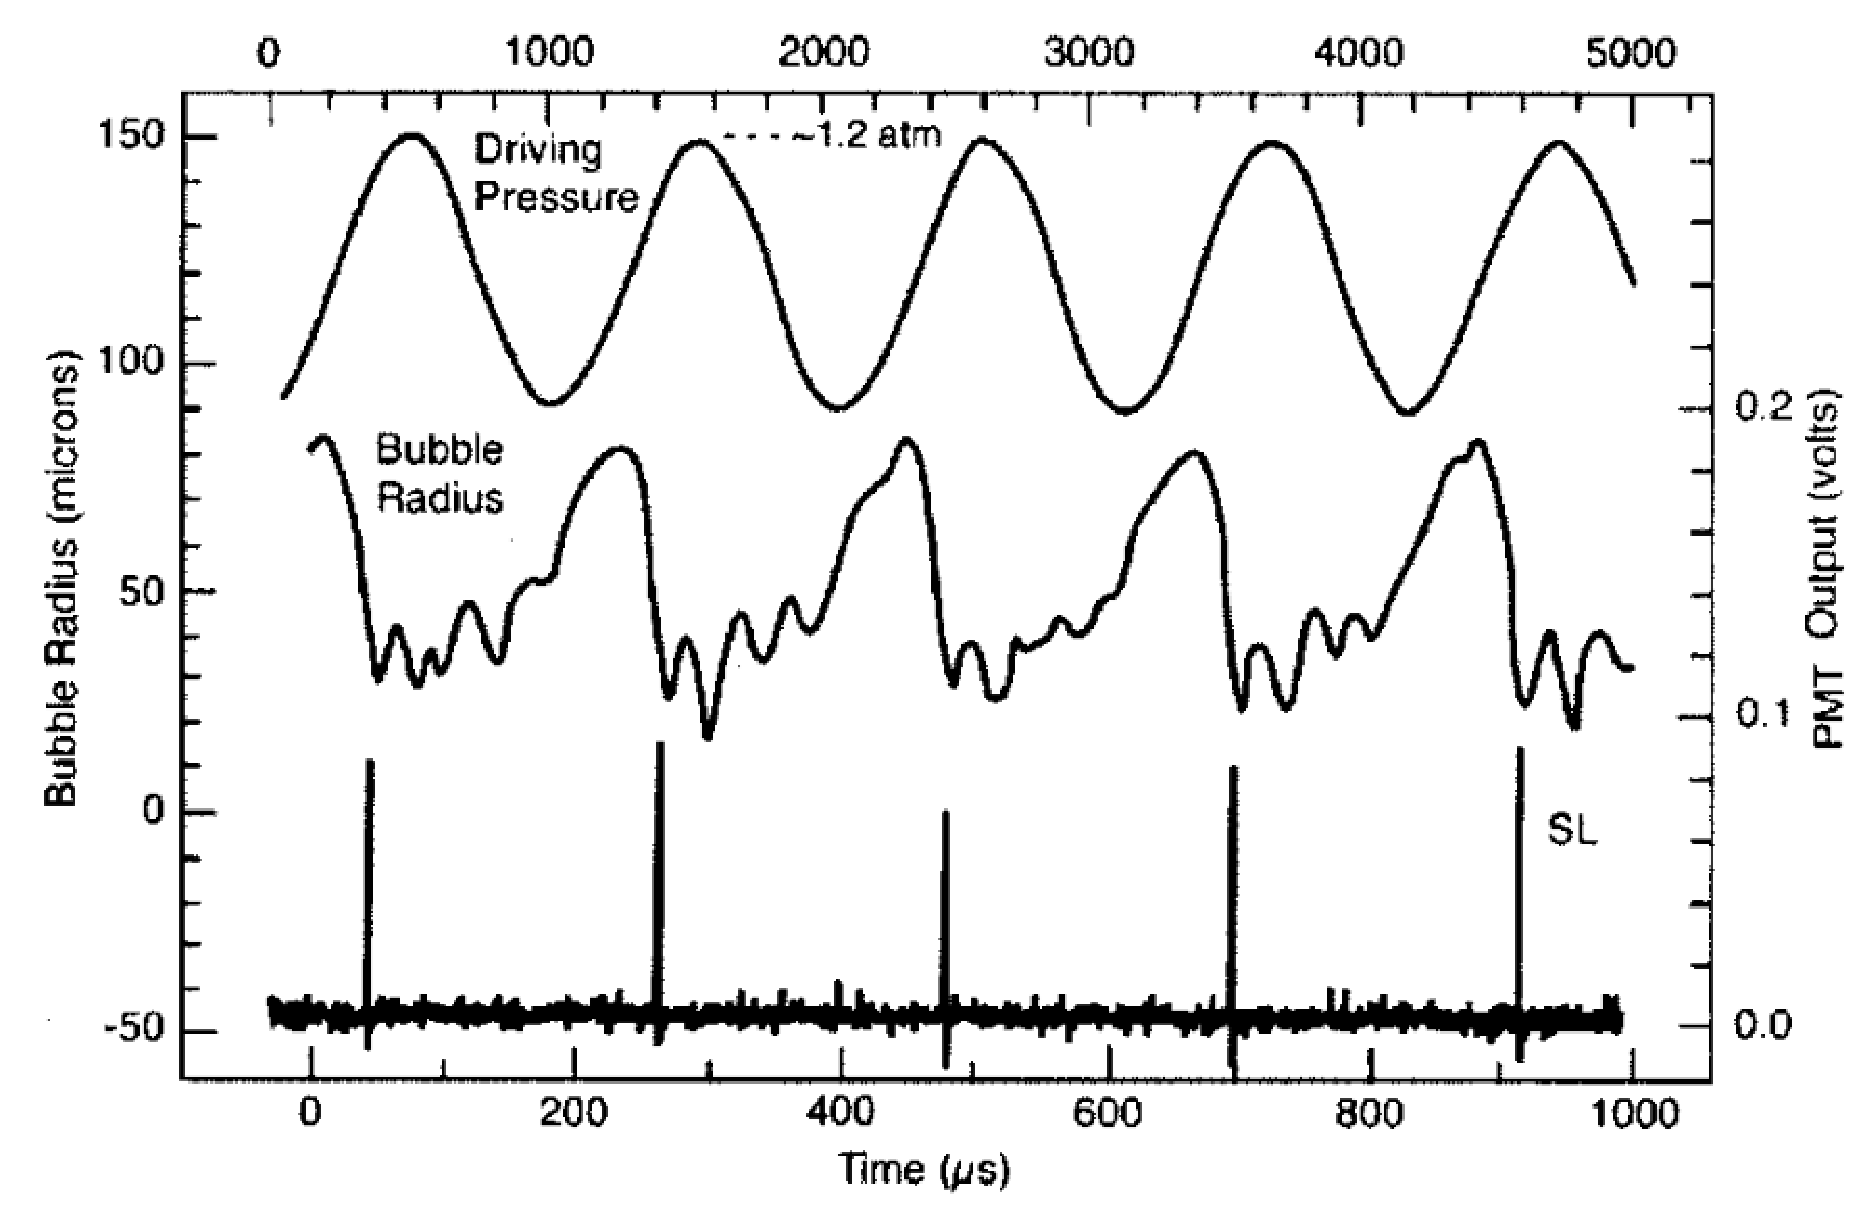
\includegraphics[width=0.7\linewidth]{figs/pulses}
    \caption{Driving pressure, bubble radius, and SL intensity as a function of time for an air bubble in water. Note that the width of the light pulse at bubble collapse is \emph{very} short. From ref. \cite{crum1994sonoluminescence}}
\label{fig:pulses}
\end{figure}

Let us now sketch SBSL more precisely. An air bubble is trapped at the center of an acoustically driven flask containing a fluid. The pressure wave in the fluid, shown as a function of time as the top curve in fig. \ref{fig:pulses}, drives the expansion and contraction of the bubble and, in turn, the gas in the bubble responds to the bubble's oscillations. Under the right circumstances, we get the very complicated non-linear response of the bubble's radius shown as the middle curve in fig. \ref{fig:pulses}. Now let's see how these dynamics lead to SBSL.

First, as the pressure decreases and becomes negative, the bubble expands gradually: surface tension and the negative pressure in the bubble tend to slow this down. Eventually the pressure is increasing again. Once it becomes positive, the bubble violently collapses to its minimum radius: during compression, the negative pressure in the bubble is very large and works with the driving pressure to rapidly accelerate the bubble's wall. The collapse is so fast that the bubble's contents are adiabatically compressed, resulting in a very large temperature in the bubble. If everything is just right, the temperature is large enough that a pulse of light is produced as shown by the bottom curve in fig. \ref{fig:pulses}. After the collapse, there is a period of \emph{after-bouncing} that continues until the pressure is negative again. 

It turns out that the light pulse is very short (only $\sim0.003\%$ of the bubble's cycle \cite{suslick2008inside}) and its spectrum depends sensitively on both the mechanical and chemical properties of the host-liquid and gas in the bubble, as well as the driving pressure and frequency \cite{brenner2002single,suslick2008inside}. The mechanical properties determine the pressure and temperature in the bubble which in turn control chemical reactions: all of these data are used to explain the light emission. For extreme enough conditions in the bubble, which occur only briefly, molecular dissociation and recombination, atomic/excited-state transitions, and electron-ion/electron-neutral atom bremsstrahlung are possible \cite{an2009diagnosing,an2008spectral,an2006mechanism,flannigan2005plasma,suslick2008inside,flannigan2006measurement}. These are now known to be the processes which emit light \cite{lohse2018bubble,yasui2018acoustic}.

Our goal in this paper is to present the simplest theory needed to understand shrimpoluminescence, though we will specialize to the related physics of a bubble undergoing SBSL in the lab as it is apparently simpler to create and characterize SBSL without involving shrimp\footnote{For example, convincing the shrimp to snap requires tickling them \cite{lohse2001snapping,versluis2000snapping,lohse2018bubble}. Besides notable exceptions \cite{tang2019bioinspired}, practically all work to study SL has not involved shrimp.}. Firstly, we will look at the problem of the fluid containing the bubble and derive the equations of motion for the bubble's wall. Nextly, we will use our results for the bubble's wall to understand the dynamics of the gas trapped in the bubble, estimate the \emph{temperature} and \emph{pressure} in the gas. We will then discuss theories presenting the mechanisms of light emission/absorption in the bubble which, combined with the temperature, allow use to calculate the bubbles light spectrum. Throughout the course of our journey, we will stick to the simplest results that still contain the essential physics we need. Connections to more advanced treatments, and their implications, are provided for completeness.

\subsection{Historical Overview}

MBSL was discovered by accident in 1933 by Marinesco and Trillat \cite{marinesco1933actions} and was subsequently characterized by Frenzel and Schultes \cite{frenzel1934luminescenz} \footnote{Neither the paper due to Marinesco et al. nor the one due to Frenzel et al. can be found by the author; in any case he can't read French or German so having the papers wouldn't be much use. As such, the story of how the effect was discovered is taken from more recent sources whose authors hopefully could read French and German \cite{brenner2002single,gaitan1990experimental,crum1994sonoluminescence}} Marinesco et al. were trying to accelerate photo development by \emph{insonating} developing fluid. They discovered that a photosensitive plate immersed in the insonated fluid became ``foggy," which they attributed to exposure to light. Shortly after, Frenzel et al. repeated the experiment and confirmed that the insonated fluid emits light in the form of a faintly glowing cloud of bubbles. 

\begin{figure}
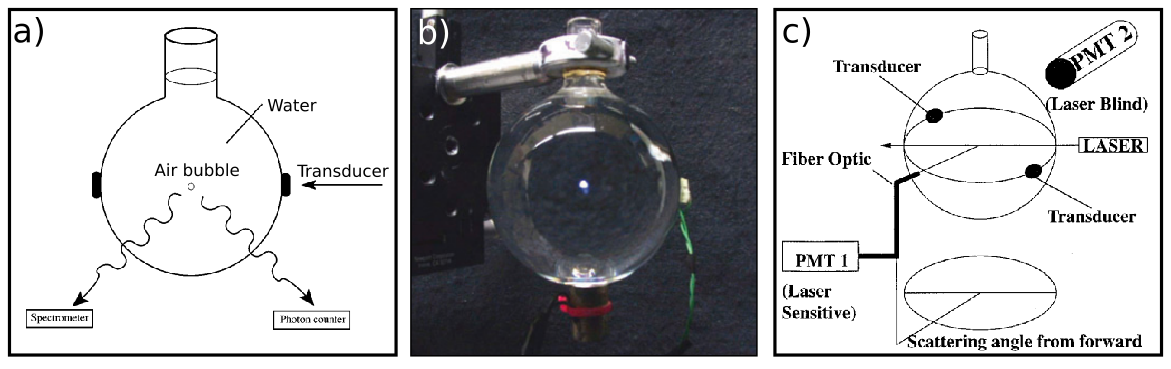
\includegraphics[width=0.95\linewidth]{figs/flask.pdf}
    \caption{(a) Schematic of a spherical ``acoustic levitation cell". The piezoelectric transducers that drive the bubble trapped in the flask are labeled in the diagram. (b) Photograph of the same. Here, the fluid is aqueous H$_2$SO$_4$ instead of water. A sonoluminescing bubble is clearly visible in the center of the flask. The photo was taken in a fully lit room with exposure time 2 s. (c) Schematic of a Mie scattering experimental setup. A similar levitation cell as (a) is shown with an added laser source and photomultiplier tubes (PMT) to analyze the scattered and emitted light. (a), (b), and (c) are from refs. \cite{brenner2002single}, \cite{suslick2008inside}, and \cite{gompf2000mie} respectively.}
\label{fig:flask}
\end{figure}

This result was not particularly surprising to the community since it had been known for a while that cavitating bubbles, e.g. those generated by the sound field, could do tremendous damage to ship's propellers \footnote{A more modern example could be my van's oil pump, which is in need of replacing.}. The discovery's impact is concisely summarized by Brenner: ``if the cloud [of cavitating bubbles] collapses violently enough to break molecular bonds in a solid, why should it \emph{not} emit photons" \cite{brenner2002single}. In fact, cavitating bubbles had been of interest to engineers working on fluid mechanics for a while. The discovery of cavitation is credited to Euler (as early as 1754) who hypothesized that if the velocity in a fluid was large enough, negative pressures could become so large as to ``break the fluid" \cite{li2015introduction,gaitan1992sonoluminescence}. Cavitation was confirmed to exist (and named ``cavitation") in 1895 by engineers studying the failure of a British Navy ship's propeller \cite{li2015introduction}. Shortly after, Lord Rayleigh wrote down and solved the differential equation for a vapor filled cavity collapsing in water (the so-called Rayleigh equation), giving the first rigorous theoretical treatment of cavitation \cite{rayleigh1917pressure,plesset1977bubble}. Rayleigh found that, for a bubble at a lower pressure than the surrounding fluid (and both pressures held constant), the bubble wall diverges during collapse. The theory has been refined considerably since then \cite{prosperetti1999old,plesset1977bubble,plesset1977bubble,brenner2002single,lofstedt1995sonoluminescing,barber1992resolving} and we will devote a large portion of this paper to this subject. Still, very little information was accessible about the light emission until the 1990's when stable \footnote{\emph{Stable} is compared with \emph{transient} when discussing cavitation. A stable bubble persists through multiple cycles of cavitation, oscillating non-linearly around an equilibrium size. Transient bubbles appear and then collapse to disappear}, single bubbles could be created and driven to emit light \cite{gaitan1990experimental,gaitan1992sonoluminescence,crum1994sonoluminescence}. With this discovery, serious interest took root. 

SBSL, unlike previous studies on MBSL, allowed very precise control and measurement of the SL process. With unprecedented experimental control, many discrepancies in previous assumptions about SL were discovered. Experiments measuring the duration of the light pulse found that it was orders or magnitude smaller than the time in which the bubble was compressed to its smallest radius \cite{barber1992resolving,barber1991observation}. This discovery implied that SL was nearly decoupled from the bubble's dynamics. New models were proposed based on \emph{converging shock waves} at the bubble's center with estimates of the temperature at the center of bubbles $\sim10^8$ K \cite{wu1993shock,greenspan1993sonoluminescence}. These very high estimates for the temperature in the bubbles led to a spark of interest more broadly: if the temperature in the bubble were really that large, then it should be possible for nuclear \emph{fusion} to occur \cite{}. An action movie featuring Keanu Reeves was made with this at the center of the plot \footnote{It is called \emph{Chain Reaction} and I am unwilling to watch it.}. and in the early 2000's, several papers were published claiming that stable nuclear fusion was possible in the lab using a method based on SBSL \cite{}. Unfortunately these results turned out to be fraudulent \cite{}. Eventually evidenced emerged that there are shape instabilities in the bubbles dynamics prohibiting converging shock-waves and severely reducing estimates for the temperature to $\sim 10,000$ K, ruling out the possibility of fusion occurring \cite{brenner2002single}. Current estimates for the temperature, which we will study in the rest of this paper, put the center of a sonoluminescing bubble between $10,000-30,000$ K \cite{flannigan2005plasma,suslick2008inside,yasui2018acoustic,an2009diagnosing,an2008spectral,an2006mechanism}.

\section{Bubble Dynamics}
In this section, we will present the theory needed to model and understand the dynamics of a bubble undergoing SBSL. We will split this into parts. Firstly, we will derive the equations of motion for the bubble's wall. Next, we will review some important experimental developments that we will then use to argue for a simple model for the dynamics of the gas in the bubble. Lastly, we will compare results of a simulated bubble to experimental data. The connection to experiment will be what allows us to calculate the temperature in real bubbles.

\subsection{The Bubble Wall}
It turns out the dynamics in SBSL are quite well described both qualitatively and quantitatively by \emph{the classical theory of bubble dynamics} \cite{prosperetti1999old,brenner2002single,prosperetti1986bubble,plesset1977bubble,suslick2008inside,yasui2018acoustic,brennen2014cavitation}. The starting point for the theory is Rayleigh's original work \cite{rayleigh1917pressure}, now expounded upon by many others. The most widely known modern work is that of Plesset \cite{plesset1977bubble,plesset1949dynamics,prosperetti1986bubble}, resulting in the so called ``the Rayleigh-Plesset" (RP) equation. The derivation assumes the host liquid is incompressible, ultimately resulting in us neglecting the effects of sound radiated by the bubble. Corrections exist that improve upon the RP equation in various ways and we will discuss this below. However, we will only derive the RP equation here and merely quote the others as they are similar in form. The field of bubble dynamics is quite mature and attempting to review it here would be out of scope of this paper; instead, the reader is referred elsewhere \cite{prosperetti1999old,brenner2002single,yasui2018acoustic,prosperetti1986bubble}. 

The RP equation is deduced from the \emph{Navier-Stokes} (NS) equations \cite{prosperetti1999old,brenner2002single,prosperetti1986bubble,plesset1977bubble,suslick2008inside,yasui2018acoustic}. The NS equations for a compressible fluid are
\begin{equation}
\begin{split}
    \rho \frac{d \bm{u}}{dt} = \rho \left[ \partial_t \bm{u}+\left(\bm{u}\cdot \nabla \right)\bm{u} \right] & =-\nabla p + \eta \nabla \left(\nabla \cdot \bm{u} \right)+\mu \nabla^2 \bm{u} + \bm{f}_B \\ 
     \partial_t \rho+\nabla\cdot(\rho \bm{u}) & = 0.
     \label{eq:NS_equations}
\end{split}
\end{equation}

Here, $\bm{u}(\bm{x},t)$ is the velocity of a fluid parcel at position $\bm{x}$ at time $t$, $\rho (\bm{x},t)$ is the fluid's density, $p$ is the pressure, $\eta \equiv \left(\xi + 2\mu/3 \right)$ is the \emph{bulk} viscosity with $\mu$ the \emph{shear} viscosity, and $\bm{f}_B$ are body forces (e.g. gravity, electrostatic forces) which are usually from external sources and will be assumed negligible from here on. The subscripts on $\partial$ denote what derivative is being taken and $\nabla$ and $\nabla^2$ have their usual meanings. The first equation is conservation of momentum for the fluid, i.e. Newton's $2^{nd}$ law; the second equation is mass conservation. The total-derivative of a moving fluid $d/dt\equiv D_t$ is sometimes called the \emph{material derivative}. In the case of velocity $D_t \bm{u}$ is the acceleration of the fluid. It records not only explicit time dependence of the fluid's velocity $\partial_t \bm{u}$ but also how the fluid's velocity varies in space as it moves past us: $\left( \bm{u}\cdot\nabla \right) \bm{u}$. The pressure term on the right hand side is to be understood as forces from the elastic energy. On the other hand, the terms $\sim \bm{u}$ are viscous (damping) terms that tend to make the velocity field spatially uniform: they vanish when the (spatial) derivatives of the velocity vanish. The bulk-viscosity term $\sim \eta$ damps radial changes in the fluids velocity (e.g. dilation/contraction) while the shear-viscosity term $\sim\mu$ resists shearing. 

Solving eqs. \ref{eq:NS_equations} is intractable. To make progress, we make some drastic approximations that are more-or-less valid for our problem. Firstly, we will assume irrational flow (i.e. $\nabla\times\bm{u}\equiv 0$) so that there is only radial motion in the liquid (i.e. $\bm{u}=u\bm{r}$). Since the flow is assumed irrotational, we can represent the velocity as the gradient of a scalar function: $u\bm{r}=\partial_r \phi \bm{r}$ \cite{jackson1999classical}. This amounts to assuming that the bubble is always spherical which seems like a rather drastic approximation but is validated experimentally. The fact that the bubble tends to remain spherical is understood by accounting for surface-tension at the liquid-bubble interface \cite{prosperetti1999old}. 

Next, we assume that the viscous terms are negligible in the bulk dynamics of the liquid. For low viscosity fluids such as water which is also nearly incompressible, this is an accurate approximation \cite{prosperetti1986bubble,prosperetti1999old,brenner2002single,plesset1977bubble}. We will account for viscosity later when looking at the bubble-liquid interface. We will also assume \emph{isentropic} and \emph{isothermal} flow, i.e. no damping and no heat flow between fluid parcels. The pressure $p$ is then determined from an instantaneous equation-of-state $p=p(\rho,T)$. In the case of SBSL, this is valid since the bubble makes up a \emph{tiny} fraction of the total volume and any heat-transport across the liquid-bubble interfacing is negligible \cite{prosperetti1999old}.

Lastly, related to the fact that the bubble is tiny, we assume that the extent of the liquid is so large compared to the bubble that we may consider the dynamics of the liquid as if there were no bubble present; similarly, we consider the dynamics of a bubble in an infinite, isotropic medium. Of course the bubble-liquid interface enters both systems as a boundary condition. 

With these simplifying assumptions (and a vector identity \footnote{$\left( \nabla \cdot \bm{u} \right) \bm{u} = \frac{1}{2} \nabla (u^2) - \bm{u}\times \left( \nabla \times \bm{u} \right)$}) we rewrite eqs. \ref{eq:NS_equations} as 
\begin{equation}
\begin{split}
     \partial_r \left[ \partial_t \phi +\frac{1}{2} \left( \partial_r \phi \right)^2 \right] & = - \frac{1}{\rho} \partial_r p  \\ 
     \partial_t \rho+ \partial_r \phi \partial_r \rho + \rho \partial^2_r \phi & = 0.
     \label{eq:NS_1D}
\end{split}
\end{equation}
We can integrate the first equation using the fact that the compressibility is negligible \cite{leighton2007derivation}.
\begin{equation}
    \int_{r_\infty}^{r} \frac{\partial}{\partial r'} \left[ \frac{\partial \phi}{\partial t} +\frac{1}{2} \left( \frac{\partial \phi}{\partial r'} \right)^2 \right] dr' = - \frac{1}{\rho} \int_{r_\infty}^{r} \frac{\partial p}{\partial r'} dr'
\end{equation}
On the left side, we take the velocity to vanish at infinity. On the right side, we assume that only the static and driving pressures, $p_\infty$ and $P(t)$ respectively, are relevant so that \cite{prosperetti1999old,prosperetti1986bubble,leighton2007derivation} 
\begin{equation}
    \partial_t \phi + \frac{1}{2}\left( \partial_r \phi \right)^2 = \frac{(p_\infty+P(t))-p(t,r)}{\rho}.
    \label{eq:press_vel}
\end{equation}
Eq. \ref{eq:press_vel} gives the pressure at coordinate $(r,t)$ in terms of the velocity of the fluid, the density, and the applied pressure. 

Now, let us assume that the velocity potential satisfies a wave equation $\nabla^2 \phi - (1/c^2)\partial_t^2 \phi =0 $ \footnote{This doesn't come from thin air. We could write the r.h.s. of eq. \ref{eq:press_vel} as the enthalpy, $h\equiv \int dp/\rho$, and similarly introduce $dh=dp/\rho$ in the first line of eq. \ref{eq:NS_1D}. Eliminating $h$ between the two and dropping small terms $\sim u/c$, we arrive at the homogeneous wave equation \cite{leighton2007derivation,brenner2002single,prosperetti1999old}.} with $c$ the speed of sound in the fluid. Again, we use incompressibility by recalling that for an incompressible fluid $c\rightarrow \infty$ which implies $\nabla^2 \phi =0$ \cite{prosperetti1999old,prosperetti1986bubble,leighton2007derivation}. Then we can ignore retardation effects and write the solution of $\nabla^2 \phi$ as 
\begin{equation}
    \phi = \frac{\psi(t)}{r}
\end{equation}
with $\psi$ the time-dependent coefficient. Now use the boundary condition for the velocity at the bubble wall, $u(R)\equiv \dot{R}$ with $R$ the bubble radius, to determine $\psi$:
\begin{equation}
    \dot{R} = -\frac{\psi}{R^2} \Rightarrow \psi = -R^2 \dot{R}.
\end{equation}  
We find $\phi(r,t) = -R^2 \dot{R}/r$. Plugging this into the left hand side of eq. \ref{eq:press_vel} and evaluating at the bubble wall, $r\equiv R$
\begin{equation}
\begin{split}
    \partial_t \phi \vert_{r=R} & = -2\dot{R}^2-R\ddot{R} \\
    \partial_r \phi \vert_{r=R} & = \dot{R} \equiv u(R)
\end{split}
\end{equation}
Finally, sticking all this together, we arrive at the Rayleigh-Plesset equation \cite{prosperetti1999old,prosperetti1986bubble,leighton2007derivation,plesset1949dynamics,plesset1977bubble}
\begin{equation}
    R\ddot{R}+\frac{3}{2}\dot{R}^2 = \frac{p_B(t)-(p_\infty+P(t))}{\rho}
    \label{eq:RP_1}
\end{equation}
with $p_B \equiv p(r=R,t)$ the pressure in the fluid at the bubble wall. The combination $p_\infty+P(t)$ is the ambient pressure \cite{prosperetti1999old,prosperetti1986bubble} which gives the pressure in the fluid in the absence of the bubble. The left hand side of eq. \ref{eq:RP_1} may be regarded as the kinetic energy (density). The right hand side is the change in enthalpy (density) due to the fluctuating bubble, i.e. the dynamics of the bubble given on the left hand side are determined by the enthalpy in the fluid due to the bubble's motion. In deriving this equation, we have assumed that the speed of propagation in the fluid is infinite. In reality, this is not true but this approximation will be very good close to the bubble (in the \emph{near-field}) where retardation effects are negligible anyway. In a similar way, we have assumed that the energy in the fluid due to distorting its volume is negligible. This approximation will be accurate near the bubble as well since the kinetic energy in this region will dominate \cite{prosperetti1999old}.

If we had not assumed incompressibility, eq. \ref{eq:RP_1} would include a term arising from the sound radiation from the bubble itself. There are practical issues with this solution however; it is third order in time and has unphysical, exponentially diverging solutions \cite{prosperetti1999old,brenner2002single,prosperetti1986bubble,lezzi1987bubble}. Both issues are solved by imposing boundary conditions on the $\ddot{R}$ term. The procedure is difficult and apparently no unique way to do it exists \cite{prosperetti1986bubble,prosperetti1988nonlinear,keller1956damping}. Instead, there is a whole family of solutions that can be derived; different variations of the RP equation, which are collectively referred to as ``Rayleigh-Plesset equations" are derived by neglecting different terms in the full compressible solution. We will discuss this again below.


We can refine eq. \ref{eq:RP_1} a little further. Since the motion in the fluid is purely radial, we expect the only relevant stresses to be normal to the bubble wall. Let's denote the radial stress in the liquid at some point $r$ by $s_r(r)=-p(r,t)+2\eta \partial_r u$. Recall, $\eta$ is the fluid viscosity from earlier. Using conservation of mass and momentum, and our expression above for the velocity, we can equate the normal stresses in the fluid to those in the bubble:
\begin{equation}
\begin{split}
    s_r(R)=-p_B-4\frac{\eta \dot{R}}{R}=-p_g+2\frac{\sigma}{R}
\end{split}
\end{equation}
where $p_g$ is the pressure in the gas and $\sigma$ is the surface tension. Solving for $p_B(t)$, we have the relation \cite{brenner2002single,prosperetti1999old,prosperetti1986bubble}
\begin{equation}
    p_B(t)=p_g(t)-\frac{1}{R}\left( 2\sigma+4\eta \dot{R} \right)
    \label{eq:p_B}.
\end{equation}
Note that in deriving the equations \ref{eq:NS_1D} we neglected the viscosity terms. This was valid since only combinations of viscosity and compressibility $\nabla \cdot \bm{u}$ appeared, both of which are assumed small. Here, however, we keep the viscosity terms coupling the bubble wall to the fluid. The RP equation becomes 
\begin{equation}
    R\ddot{R}+\frac{3}{2}\dot{R}^2 = \frac{1}{\rho} \left[ \Delta p(t)-\frac{1}{R}\left( 2\sigma+4\eta \dot{R} \right)-P(t) \right]
    \label{eq:RP_2}
\end{equation}
with $\Delta p = p_g(t)-p_\infty$ the deviation of the pressure inside the bubble from the static pressure. With the above assumption that the compression is adiabatic, the conditions inside the bubble are decoupled from the liquid (besides the coupling through the RP equation) and we may regard $p_g(t)$ in the bubble as a given quantity to be determined from an equation of state. Recall $P(t)$ is the time-dependent part of the pressure in the absence of the bubble: we may regard this as an external pressure from e.g. a driving stress. In SBSL, this is from the transducers driving the flask and $P(t)$ is an acoustic plane wave. Keller and coworkers showed that the modification required to the RP equation is the replacement $P(t) \rightarrow P_0 \sin(\omega t)$ \cite{keller1980bubble}. 

%\begin{figure}
%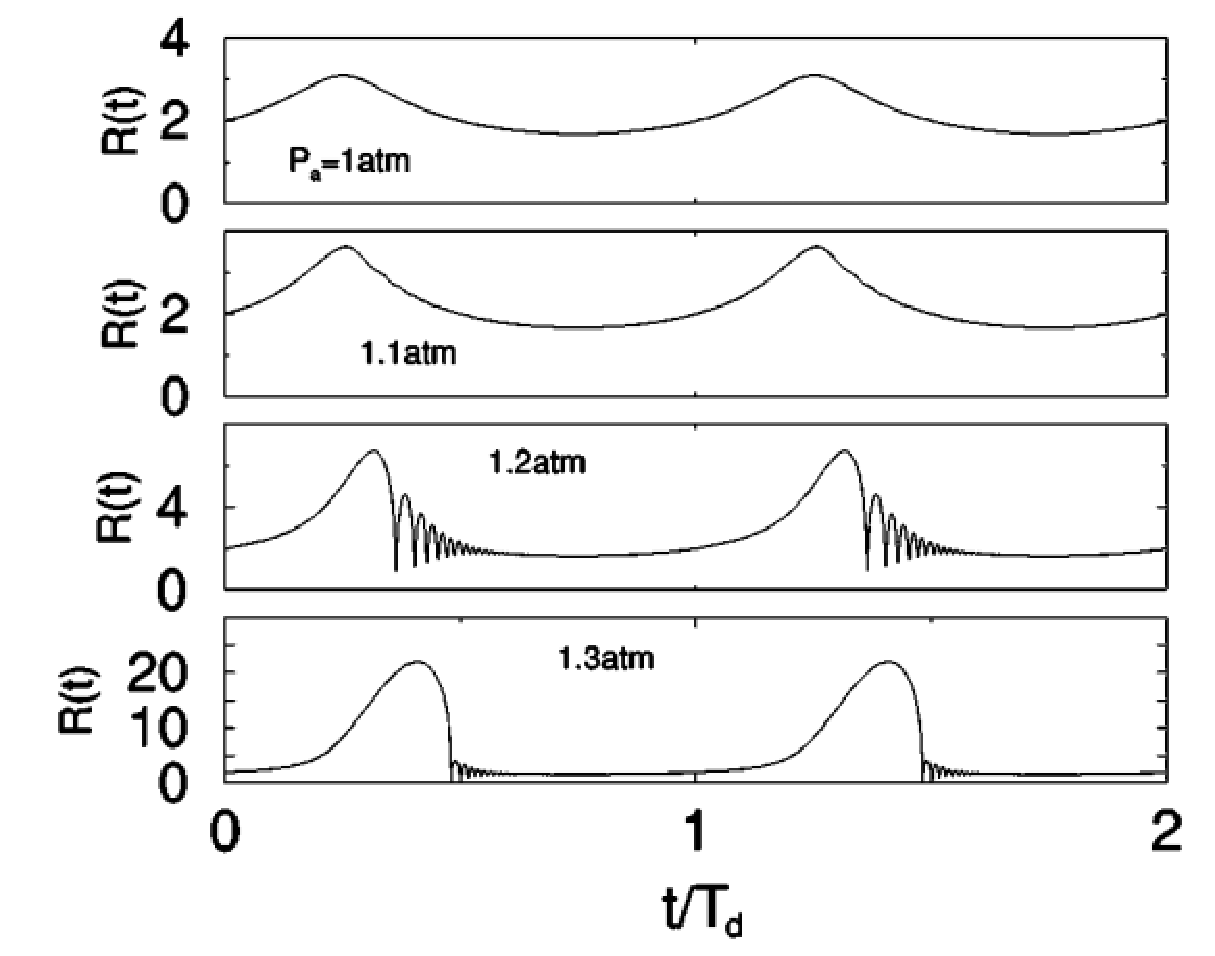
\includegraphics[width=0.5\linewidth]{figs/bubble_radius_2.pdf}
%    \caption{Solutions to eq. \ref{eq:RP_2} for different driving pressures. For driving at 1 atm, the dynamics are a simple pulsating bubble. For larger driving pressure, e.g. 1.2 atm, we observe strongly non-linear behavior exhibiting cavitation and afterbounces. For even larger driving pressure, we encounter the regime where SBSL begins to occur. From ref. \cite{brenner2002single}}
%\label{fig:bubble_radius_2}
%\end{figure}

The RP equation (eq. \ref{eq:RP_2}) is pretty but its analytical solution is intractable. Direct solutions of the RP equation or its variants are done numerically using e.g. Euler or Runge-Kutta methods \cite{yasui2018acoustic,yasui2015dynamics}. It is no great challenge computationally. For now, let's see what we can understand analytically by making some more approximations. If we linearize in the bubble's radius $R(t)\approx R_0 \left( 1+x(t) \right)$ with $x(t) \ll 1$, we can derive a forced harmonic oscillator equation for $x(t)$ \cite{brennen2014cavitation,yasui2018acoustic}. However, the low driving amplitude regime where this method is valid is irrelevant to SBSL so we won't pursue it here. Instead, we can look at the interval where the bubble wall's velocity is very large, called \emph{The Rayleigh Collapse}; the right hand side of eq. \ref{eq:RP_2} will be much smaller than the $\dot{R}^2$ term and we may neglect it \cite{rayleigh1917pressure,plesset1949dynamics,prosperetti1999old,brenner2002single}. 
Rayleigh looked at the same problem, i.e. a cavitating void in water:
\begin{equation}
    R\ddot{R}+\frac{3}{2}\dot{R}^2=0
    \label{eq:Rayleigh}
\end{equation}
and found the solution to be $R(t)\sim\left(t_*-t\right)^{2/5}$ \cite{brenner2002single}, with $t_*$ the time of collapse. The velocity, $\dot{R}\sim\left(t_*-t \right)^{-3/5}$, diverges as the bubble collapses. This observation is what lead to Rayleigh's argument for the origin of cavitation damage to ship's propellers. %Yasui gave a rather elegant heuristic explanation for the origin of \emph{cavitation} in a fluid that is worth stating here \cite{yasui2018acoustic}. Consider the mass flowing through concentric shells around a bubble, $4\pi R_i^2 v_i \rho$. For a source free field, we require that neighboring shells satisfy conservation of mass: $4\pi R_1^2 v_1 = 4\pi R_2^2 v_2$. For $R_2 > R_1$, we see that $v_1/v_2 = \left(R_2/R_1\right)^2$. The velocity for a smaller radius is always larger, diverging towards the origin.

In reality, the bubble's velocity does not become infinite and, in the case of \emph{stable} SBSL, the radius remains finite at all times. In the full RP equation (eq. \ref{eq:RP_1}) the only term capable of compensating the bubble wall's motion is the diverging pressure inside the bubble itself \cite{brenner2002single}. Applying the same analysis to the family of solutions derived when including the bubble's sound radiation, it turns out that the most important term for slowing the bubble wall's diverging velocity is $\propto\dot{p}_g$. Keeping only this term, we arrive at the most popular variant of the RP equation \cite{lofstedt1995sonoluminescing,barber1997defining}:
\begin{equation}
    R\ddot{R}+\frac{3}{2}\dot{R}^2 = \frac{1}{\rho} \left[ \Delta p(t)-\frac{1}{R}\left( 2\sigma+4\eta \dot{R} \right)-P(t) +\frac{R}{c} \dot{p}_g \right].
    \label{eq:RP_3}
\end{equation}
This equation is only slightly more complicated than the RP equation (eq. \ref{eq:RP_2}), the only change being the added term $\propto \dot{p}_g$ which is determined from solving the decoupled problem of the gas inside the bubble. The observed error between this equation and experiment is only significant in the interval during bubble collapse and even still, results of solving this equation are quantitatively in good agreement with measurements of the bubble's radius \cite{brenner2002single}. 

Above, we assumed that the bubble always remains spherical. Of course this isn't always true and \emph{shape-instabilities} occur for the right combinations of mechanical properties and driving force/frequency. Usually shape-instabilities destroy the bubble and kill SBSL so we won't focus on these isues here. We will always assume we are in a parameter-regime where SBSL occurs. The reader is referred to one of several reviews on the \emph{phase-space} of SBSL for more info \cite{yasui2018acoustic,brenner2002single,hilgenfeldt1999sonoluminescence,an2009diagnosing}. 


\subsection{The Bubble's Interior}
The theoretical progress on the bubble's interior since the discovery of SBSL in the late 1990's \cite{gaitan1992sonoluminescence} follows two paths \cite{brenner2002single,suslick2008inside,yasui2018acoustic}: (i) model calculations based on the RP equations and an equation of state for the pressure (from which we may calculate the temperature) are used to try to reproduce the easily measurable dynamics of the bubble. (ii) We can model the light emission itself and compare our calculation to spectroscopic measurements of SBSL \cite{hiller1992spectrum,brenner2002single}. Obviously these are related topics, but the distinction in the context of SBSL is important as we will now see.

Most early progress on the bubble's interior depended on the former method: if we predict the right dynamics, then we might know the correct pressure and temperature in the bubble. These data are then used to try to describe the light emission. This was preferred over studying the emitted spectra directly as careful measurements resulted in an almost featureless spectrum that could not be explained \cite{hiller1992spectrum}. Calculating the dynamics of the bubble's wall from the RP equations (eq. \ref{eq:RP_2} or eq. \ref{eq:RP_3}) requires the pressure inside the bubble as input. We would like to find a suitable form for $\Delta p(t) \sim p_g(t)$ in the RP equations that reproduces the measured radius-time curve $R(t)$ for a stable cavitating bubble. It turns out that this is a very complicated problem: gas diffusion and rectification (one-directional diffusion) between the bubble and liquid vary the number of particles present and, to make things worse, the conditions inside the bubble facilitate chemical reactions between the air and water-vapor changing the properties of gas dynamically \cite{brenner2002single}. Brenner et. al elegantly summarized the significance of this problem \cite{brenner2002single}: ``one of the exciting features of modern research on SBSL is that it is a testing ground for how well mathematical models can deal with such a complicated situation"

The other method to understand the bubble's interior is its light spectrum. For the first decade or so, SBSL experiments were done using partially degassed\footnote{Degassing lowers the ambient pressure, making it easier for bubbles to form.} water as the liquid medium \cite{suslick2008inside,brenner2002single,gaitan1992sonoluminescence}. Careful measurements of the emission from SBSL in water resulted in an almost featureless spectrum and attempts to fit it as black-body radiation were not sucessful \cite{hiller1992spectrum}. It was later discovered that SBSL is volume emission, indicating that a black-body is not valid anyway \cite{hilgenfeldt1999simple,hilgenfeldt1999sonoluminescence}. Little progress was made on this front for quite some time \cite{brenner2002single}. The utility of analyzing the light spectrum of SBSL in water is succinctly described by Suslick \cite{suslick2008inside}: ``because of the inherent ambiguity associated with the analysis of featureless spectra of unknown origin, a more rigorous explanation is unlikely to be generated". 

Some attempts were made to measure SBSL using non-aqueous host liquids e.g. alcohols, silicone oils \cite{weninger1995sonoluminescence,barber1997defining}, but experiments with air bubbles were not very successful \cite{barber1997defining}. Eventually, different gases were tried in water. Recall, air is $\sim 80\%$ N$_2$, $\sim 20\%$ O$_2$, and $\sim 1\% $ Ar. Considering the relatively large content of O$_2$ and N$_2$, degassed water \emph{regassed} with N$_2$ or O$_2$ or a mixture were checked first and found not to produce SBSL \cite{hiller1994effect}. What was discovered was that a small amount of noble-gas was required for SBSL to occur \cite{barber1997defining,hiller1994effect,brenner2002single}. A result of this work was the \emph{argon rectification hypothesis} \cite{lohse1997sonoluminescing,brenner2002single,yasui2018acoustic,suslick2008inside}. The hypothesis claims that all species in the air inside the bubble besides argon are gradually ejected from bubble's interior until all that remains is pure argon. The theory is based on the fact that, at the elevated temperatures and pressures inside the bubble, dissociation of O$_2$ and N$_2$ into radicals is possible. These species then react with the water vapor radicals to form species that are soluble in the host fluid. As the pressure becomes very large during the compression stage of SBSL, the soluble materials leave the bubble and do not re-enter since their solubility in water is enormous compared to the Ar content of the bubble \cite{lohse1997sonoluminescing}. Over many cycles, the contents of an air bubble in water become nearly pure argon. Moreover, it was hypothesized that the SL would be much more intense when the contents of the bubble are a pure inert gas: if the contents were e.g. molecules, bond breaking/formation would alter the pressure of the gas, ultimately reducing the temperature and reducing the amount of light production \cite{brenner2002single,yasui2018acoustic,lohse2018bubble,suslick2008inside}. This mechanism has been used to explain the relatively weak light, i.e. the low temperature, in MBSL: the bubbles are transient and cannot remove a significant amount of O$_2$ or N$_2$ over a single cycle. The current belief is that the contents of a bubble undergoing SBSL in water are (nearly) pure argon after $\sim 10^3$ cycles \cite{brenner2002single,yasui2018acoustic}.  

Still, most studies continued to use water as the host liquid until it was realized that SBSL in aqueous H$_2$SO$_4$ produces light $10^3$ times brighter than in water, allowing more precise measurements of the light spectrum \cite{flannigan2005plasma,flannigan2006measurement}. The mechanical properties in aqueous H$_2$SO$_4$ allow stable SBSL with a larger bubble radii than in water, increasing the emitting volume. More importantly, new measurements revealed the phase space of SBSL in aqueous H$_2$SO$_4$ included a much larger range of pressure than water. SBSL in aqueous H$_2$SO$_4$ could be driven at very low pressure, leading to much lower temperature bubbles, while driving at large pressure led to conditions similar to SBSL in water. 

Careful experiments revealed that the spectrum depended critically on the noble-gas content and driving pressure. Suslick et. al measured the different emission spectra from Ar, Xe, and Kr bubbles in aqueous H$_2$SO$_4$, driven to have similar conditions to those in an air bubble in water \cite{flannigan2005plasma,flannigan2006measurement,suslick2008inside}. Importantly, they were able to identify spectral lines from Ar$^+$, Xe$^+$, and Kr$^+$ excited state transitions, proving that the core of the bubble is plasma. Perhaps equally as crucially, they found the absence of emission lines from components of aqueous H$_2$SO$_4$ vapor \cite{suslick2008inside,flannigan2006measurement,flannigan2006measurement}: the plasma contained only the noble-gas, experimentally confirming the argon rectification hypothesis. The spectra at different pressures were in very good agreement with detailed calculations of emission from noble-gas plasmas \cite{an2009diagnosing,an2008spectral}. This work also explained why the spectrum in water is featureless (i.e. has no emission lines). The larger pressure in SBSL in water results in an increased collision rate between particles, broadening the spectral lines \cite{an2009diagnosing,suslick2008inside,flannigan2005plasma,flannigan2006measurement}.

This argon rectification hypothesis greatly helped to refine models for the gas dynamics in the bubbles and confirmed why simple models usually work well \cite{suslick2008inside,brenner2002single}. With this in mind, we choose only to focus on results known to be relevant to the dynamics of a bubble undergoing SBSL. Excellent books and modern reviews on modeling the gas dynamics exist elsewhere \cite{brenner2002single,yasui2018acoustic,brennen2014cavitation}. We will hold off on discussing the plasma until a later section. 

\subsection{Gas Dynamics}
Of course the most straightforward way to model the gas dynamics in the bubble is through direct solution of the Navier-Stokes equations for the gas \cite{brenner2002single}. In fact, serious quantitative predictions of the conditions of the bubble's interior still take this path \cite{an2006mechanism,an2008spectral,an2009diagnosing,flannigan2005plasma,flannigan2006measurement}. With simplifying assumptions, equations of motion with varying degrees of sophistication can be derived for the gas and the system of gas dynamical equations and the RP equations are solved numerically. The discussion proceeds in much the same way as deriving the RP equations above but is slighlty more complicated \cite{brenner2002single,yasui2018acoustic}, so we will omit it. An important aspect of these studies is the understanding of why relatively simple models work quite well. 

We will highlight the salient features before introducing a simple model for the gas that will enable us to gain some physical understanding analytically. An especially important result of direct numerical solution of the gas dynamics was (theoretical) confirmation of the argon rectification hypothesis, reducing the possible gas dynamical models to those applicable to a monatomic gas. Various other models fully including dissipation and heat transport into/out of the bubble showed that the bubble's compression is, to a good approximation, adiabatic and quasistatic. Before we turn to discuss a model for the gas dynamics, let us pause to mention that another theoretically appealing method for modeling the gas dynamics is \emph{molecular dynamics}. While this method is attractive for a number of reasons, practical calculations containing realistic numbers of particles aren't possible, limiting the applicability \cite{brenner2002single}.

Recalling that the bubble is (almost) purely noble-gas, a simple but reasonable model for the gas dynamics is that of an adiabatically, quasistatically compressed ideal\footnote{Actually a \emph{Van der Walls} gas model is better, but we will sneak this aspect in later. The modifications to the result for an ideal gas are simple \cite{sivasubramanian2002temperature}.} gas \cite{brenner2002single}. Let us remind ourselves what the pressure is. Suppose that we have a volume, $V$, of an ideal gas containing $N$ particles at a temperature $T$. The ideal gas law tells us the equation of state is $PV=Nk_BT$ with $k_B$ Boltzmann's constant. Since we are assuming adiabatic compression, the second law of thermodynamics is $dU=-PdV$ with $U$ the internal energy in the gas. We may use the equipartition theorem to write $dU=N f k_B dT/2$ with $f$ the number of degrees-of-freedom per particle \cite{schroeder1999introduction}. Recall that for an ideal gas the specific heat at constant volume is $C_V = N f k_B/2$ and at constant pressure is $C_P = C_V+N k_B$, with $C_P/C_V = 1+2/f \equiv \gamma$. For a noble-gas, $f=3$ and $\gamma=5/3$. Now we can use the second law of thermodynamics to write $C_V dT = -P dV$. From the equation of state, we have
\begin{equation}
    dT = \frac{PdV+VdP}{Nk_B}=\frac{PdV+VdP}{C_P-C_V}.
\end{equation}
Inserting $dT$ into the second law and simplifying, 
\begin{equation}
    \frac{dP}{P}=-\left(\frac{C_P}{C_V}\right) \frac{dV}{V} = -\gamma \frac{dV}{V}.
    \label{eq:dP}
\end{equation}
Integrating eq. \ref{eq:dP}, we find 
\begin{equation}
    P_2 = P_1 \left(\frac{V_1}{V_2}\right)^\gamma
\label{eq:P}
\end{equation}
where $P_2$ is the pressure in a gas at volume $V_2$ that was initially contained in a volume $V_1$ at pressure $P_1$. Importantly we have not made any assumptions about the shape of the container. 

Let us now connect this to the problem of SBSL. In our case, we assume that our bubble has an ambient radius $R_0$ where the pressure is at its equilibrium value, $p_0$. The volume occupied by the gas is $V_0 =  4/3 \pi R_0^3$. We know that $p_0=p_\infty+2\sigma /R$ from earlier. What we want to calculate is the pressure in the gas as a function of the bubble's instantaneous radius $R(t)$ determined from the RP equations (eq. \ref{eq:RP_2} or eq. \ref{eq:RP_3}). Earlier we called the pressure in the gas $p_g(t)$ and we will stick with this here. Plugging these into eq. \ref{eq:P}, (and sneaking in a modification) we arrive at a very commonly used equation in the context of SBSL \cite{brenner2002single,lofstedt1995sonoluminescing,barber1997defining,lofstedt1993toward,hilgenfeldt1999simple}:
\begin{equation}
    p_g(t) = \left( p_\infty+2\frac{\sigma}{R_0} \right) \left[ \frac{R_0^3-h^3}{R^3(t)-h^3} \right] ^ \gamma
    \label{eq:p_g}
\end{equation}
The new variable $h$ that was added willy-nilly is called the \emph{Van der Walls hard-core radius} and its purpose is to make sure that, if the bubble collapses so strongly that its contents become incompressible (i.e. $R(t)\rightarrow h$), the pressure diverges \cite{lofstedt1993toward,brenner2002single}. Eq. \ref{eq:p_g} can be inserted into an RP equation which can then be integrated numerically to determine the bubble's dynamics. 

Our physical intuition tells us why eq. \ref{eq:p_g} is sensible during the bubble's collapse: the bubble wall's velocity is fast and very little heat can flow out during compression. Detailed calculations starting from the full NS equations further tell us that the gas dynamics in the bubble can be regarded as \emph{quasistatic} \cite{brenner2002single}. During the expansion and after-bounce stages of the bubbles cycle, which comprise its majority, the gas dynamics should instead be regarded as \emph{isothermal}. This is true because, when the bubble's velocity is on the order of the heat diffusion timescale, the temperature throughout the bubble is nearly equal to that in the liquid \cite{prosperetti1999old,brenner2002single,yasui2018acoustic}. The relevant modifications to eq. \ref{eq:p_g} turns out to be replacing $\gamma\rightarrow 1$. A neat way of including both isothermal and adiabatic gas dynamics is continuously varying the exponent, $\gamma$ in eq. \ref{eq:p_g}, between its adiabatic and isothermal values, $C_P/C_V$ and $1$, respectively. A summary of this work is given in refs. \cite{brenner2002single} and \cite{prosperetti1999old}. It turns out that this process doesn't result in better quantitative predictions since, during the assumed isothermal part of the process, dissipation becomes important \cite{brenner2002single}. A simple alternative is choosing a constant exponent somewhere between the adiabatic $\gamma=5/3$ and isothermal $\gamma=1$ values \cite{hilgenfeldt1999simple}. It is also possible to include heat and mass diffusion in simple model forms and these do give slightly improved quantitative agreement with experiment; however the simpler form given in eq. \ref{eq:p_g} gives close to the correct dynamics (see fig. \ref{fig:bubble_radius_1}). More advanced solutions using the full gas dynamical equations are qualitatively similar \cite{brenner2002single,yasui2018acoustic}.

Now recall that one of main goals of modeling the bubble dynamics in SBSL was to calculate the temperature inside the bubble in order to model the light emission. Following similar steps to deriving $p_g(t)$, we can write down an equation for the temperature $T$ \cite{barber1997defining,brenner2002single}:
\begin{equation}
    T(t) = T_0 \left( \frac{R_0^3-h^3}{R^3(t)-h^3} \right)^ {\gamma-1}.
    \label{eq:T(t)}
\end{equation}
Earlier, we said that during the bubble's after-bounces and expansion, the gas dynamics is isothermal; then we take $T_0$ to be the temperature of the liquid. The RP equation, eq. \ref{eq:RP_3}, combined with the gas dynamical equation, eq. \ref{eq:p_g}, and the known liquid and gas properties $\eta$, $\sigma$, and $h$, can be used to calculate the dynamics of an acoustically driven bubble, giving us the time-dependence of the pressure and temperature in the bubble. 

\subsection{Bubbles in the Lab}
\begin{figure}
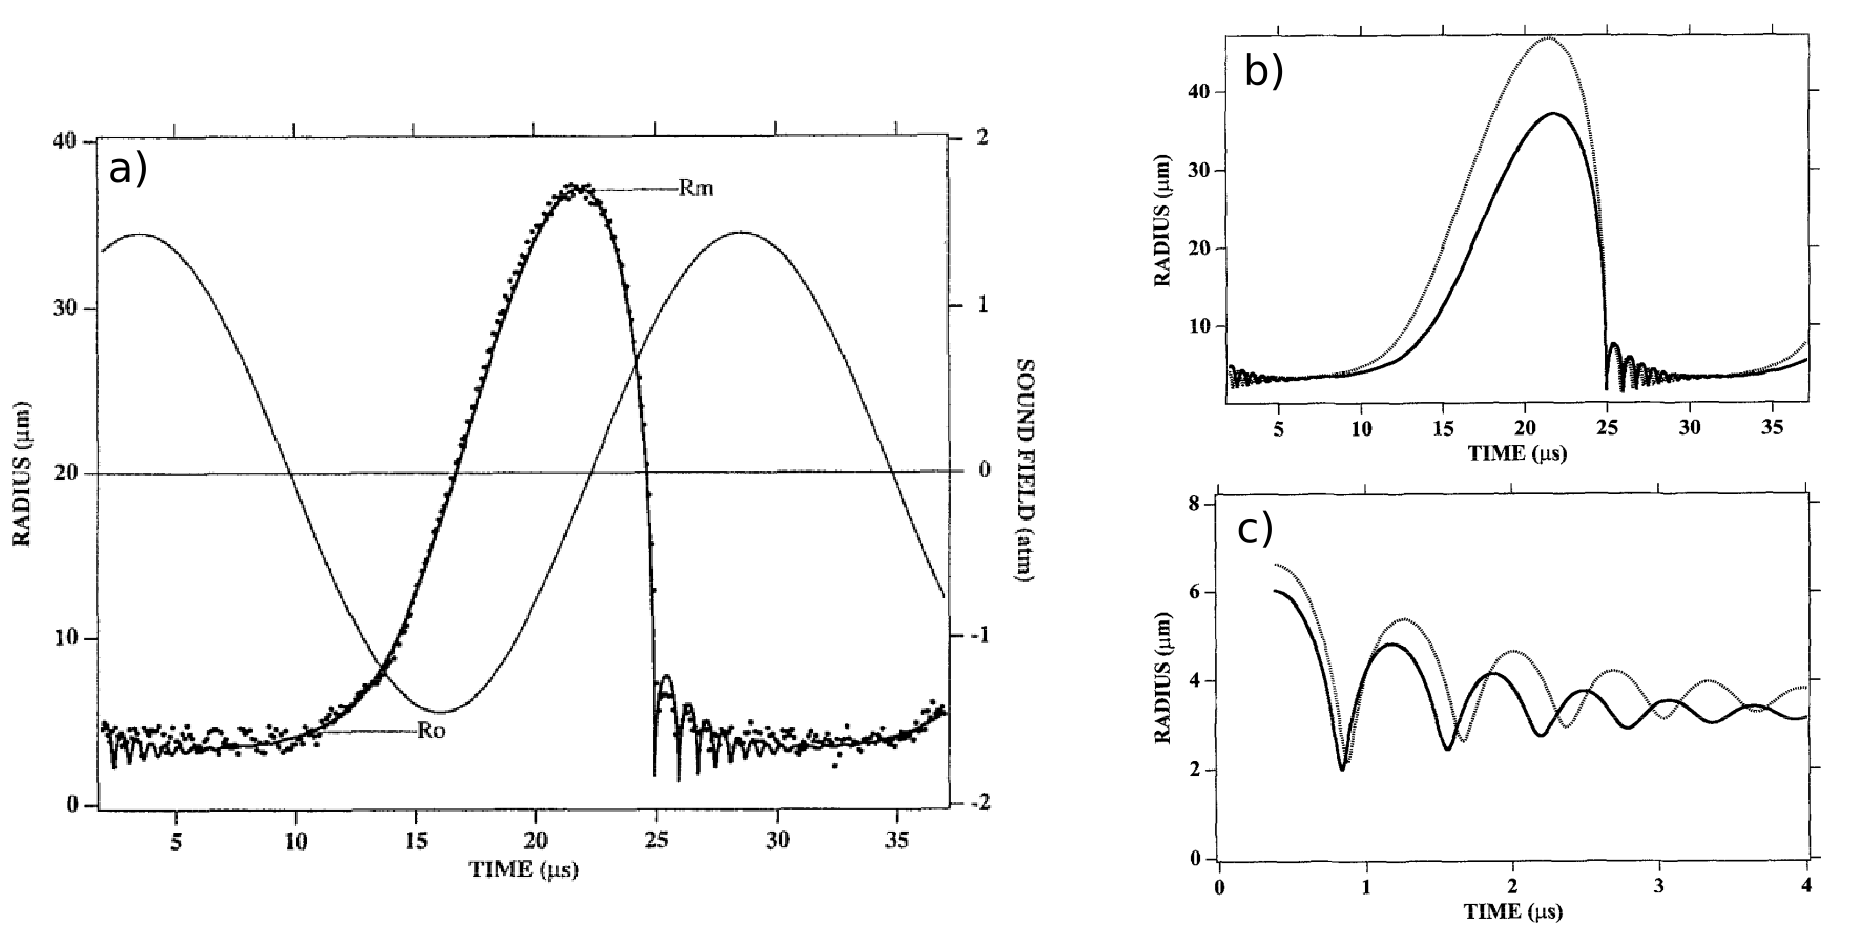
\includegraphics[width=0.9\linewidth]{figs/bubble_radius_1.pdf}
    \caption{Numerical solution of the RP equation variant eq. \ref{eq:RP_3} with the gas dynamics given by eq. \ref{eq:p_g} compared to Mie scattering results \cite{barber1997defining,barber1992light}.}
\label{fig:bubble_radius_1}
\end{figure}

Creating stable, single bubbles in a laboratory experiment is not particularly challenging and can be done with standard and low-cost materials \footnote{Actually, the phase-space for SBSL is ``small". The coordinates being driving amplitude, driving frequency, fluid composition, temperature, ambient pressure, gas content and composition, etc... What we are claiming is simple is the experimental setup once the correct parameters are identified.}. A typical experimental setup is shown in fig. \ref{fig:flask}. Since we are mainly concerned with the explaining the light emission process itself, we will only sketch the experimental setup; it can be summarized as follows \cite{lentz1995mie,gaitan1990experimental,gaitan1992sonoluminescence,gompf2000mie,brenner2002single,yasui2018acoustic,brennen2014cavitation,suslick2008inside}. A suitable sample of liquid is placed into a flask. Coupled to the outside of the flask are piezoelectric transducers of some sort. The piezos are driven by a sinusoidal function generator to excite an acoustic resonance of the flask: a typical flask is a few cm across with a resonance at $\approx 20$ kHz \cite{brenner2002single}. The frequency is chosen to form a pressure \emph{antinode} at the center of the flask.

%Let us take a brief aside: in deriving the RP equations, we assumed the center of the bubble was stationary. Actually, this is what we want in an SBSL experiment and it is worth discussing under what conditions this is true. In an ideal, incompressible fluid the net force acting on a bubble may be written as 
%\begin{equation}
%    \bm{f}=-\int_{\partial \Omega} p \bm{n} dA = -\int_\Omega \nabla p dV
%\end{equation}
%Here, $\bm{f}$ is the net force, $p$ is the pressure at the bubble's surface, $\bm{n}$ is the unit normal vector point out of the bubbles surface, and $\partial \Omega$ is the bubble's boundary with $\Omega$ the bubble's domain. The last term is due to an application of Gauss's theorem. Bjerknes \cite{bjerknes1909kraftfelder} took $\nabla p \equiv \nabla p(r=0,t)$ to be constant and averaged over one period of oscillation to find 
%\begin{equation}
%    \bm{f} = -\frac{4}{3}\pi \langle R^3 \nabla p \rangle.
%    \label{eq:Bj_force}
%\end{equation}
%This is the so called \emph{Bjerknes force}. The point is that if the bubble is located at a pressure extrema, e.g. the antinode at the center of the flask, then this force should vanish and the bubble will remain stationary, an essential result for SBSL experiments.

%Some authors have looked at corrections to the bubble's dynamics in the presence of buoyancy, which cause translational motion even for vanishing Bjerknes force. The result is the bubble oscillates around an equilibrium position near but away from the center of the flask \cite{matula2000single,matula1997bjerknes,matula1999inertial}. The translational motion of the bubble leads to shape distortion which is believed to suppress SL; this is confirmed by SBSL experiments in microgravity resulting in larger intensity light production \cite{matula2000single}.

The typical driving pressure relevant to SBSL ($\sim 1.5$ atm) is too small to cause bubbles to form spontaneously in the flask \cite{brenner2002single}. Instead, the bubble is usually seeded somehow. In the original work of Gaitan, an air bubble was injected using a needle and syringe through a small hole in the flask's seal \cite{gaitan1992sonoluminescence}. More recently, seeding methods involve shooting a small jet of water into the flask (like our shrimp friends!) or blasting the water with a laser to boil a small volume \cite{suslick2008inside,yasui2018acoustic}. The later method is preferred as it enables more precise control over the initial bubble's radius. 

Now that we know about how single, stable bubbles are formed in the lab, we can discuss two experimentally accessible quantities that have turned out the be the most important: (i) The bubble's radius may be measured by \emph{Mie scattering} and compared directly to solutions of the RP equations \cite{barber1992light,barber1997defining,brenner2002single}. This can tell us about the temperature and pressure in the bubble. (ii) The other quantity of interest is the light spectrum which contains information on the bubble's contents: in principle, we can learn about temperature and pressure inside the bubble, with spectral lines telling us about the matter content \cite{hiller1992spectrum,hilgenfeldt1999simple,flannigan2005plasma,flannigan2006measurement}. As we will see, it is not simple to understand the light spectrum and we will devote a section of this paper to this topic. For now, let us see what measurements of the bubble's dynamics have told us. 

%Mie scattering measurements scatter a laser off a bubble and analyze the scattered intensity. Assuming the bubble is a homogeneous dielectric sphere \cite{jackson1999classical}, the angular distribution of light scattered from the bubble at \emph{fixed radius} and the time-dependent scattering off the bubble at \emph{fixed angle} allow use to accurately measure the bubble's radius as a function of time \cite{brenner2002single}. A typical Mie scattering experiment is shown in fig. \ref{fig:flask} (c). Two important sources of experimental error are changes to the dielectric properties of the bubble during its cycle \cite{} and the fact that cavitating bubbles can emit an outward going shock \cite{}: some light scatters off the outward-going spherical wave too \cite{}. Both effects are largest during the SL period of the bubble's cycle, leading to an important source of error when fitting the calculated $R(t)$ curve \cite{}. 
Mie scattering measurements scatter a laser off a bubble and analyze the scattered intensity. Assuming the bubble is a homogeneous dielectric sphere \cite{jackson1999classical}, the angular distribution of light scattered from the bubble at \emph{fixed radius} and the time-dependent scattering off the bubble at \emph{fixed angle} allow use to accurately measure the bubble's radius as a function of time \cite{brenner2002single}. A typical Mie scattering experiment is shown in fig. \ref{fig:flask} (c). Parameters used to calculate the gas dynamics in the bubble are fit to the measured radius to build a full model of the dynamics. In the case of eq. \ref{eq:p_g}, the quantity to fit is $R_0$. The results of a calculation using eq. \ref{eq:p_g} combined with the RP variant eq. \ref{eq:RP_3} and fit to experiment are shown in fig. \ref{fig:bubble_radius_1} (a). The ambient ambient radius is $R_0=1.45$ $\mu$m for driving pressure $P_0=1.45$ atm \cite{barber1997defining,barber1992light}. Note the large change in the calculated dynamics for relatively small changes in $R_0$ and $P_0$ in Fig. \ref{fig:bubble_radius_1} (b) and (c). 

More accurate treatments of the gas dynamics from numerically solving the gas's NS equations are qualitatively in good agreement with these simpler model calculations \cite{brenner2002single,yasui2018acoustic}. They are, however, in better quantitative agreement when their results are used to calculate the light spectrum \cite{an2009diagnosing,an2008spectral,an2006mechanism,flannigan2005plasma,flannigan2006measurement,suslick2008inside}. Let us turn to discuss the light's spectrum now.

\section{Let there be light!}
An important requirement for models of the light emission is \emph{local thermodynamic equilibrium} (LTE). LTE is required for many reasons, foremost being the definition of temperature. LTE is expected to be true in a bubble undergoing SBSL since the particle density, $\sim 10^{28}/m^3$, and temerature, $\sim 10^4$ K, guarantee collisions between particles occur so frequently that equilibrium is ensured \cite{brenner2002single,hilgenfeldt1999sonoluminescence,yasui1999mechanism}.

\emph{Any} ensemble of atoms at a well defined temperature will emit radiation according to Planck's law. In the case of SBSL, we will look for corrections due to interactions of the emitted photons with atoms on the way out of the bubble \cite{hilgenfeldt1999sonoluminescence}. Since we are assuming LTE, the intensity of emitted radiation depends instantaneoisly on the temperature-time curve, $T(t)$, that we just learned how to calculate. Planck's law gives the energy radiated per unit-time and unit-volume, $I_B$, \cite{schroeder1999introduction}
\begin{equation}
    I_{B}(\lambda;T(t))=\frac{2 h c^2}{\lambda^5}\frac{1}{\exp(hc/\lambda k_B T(t))-1}.
\end{equation}
The subscript $B$ is to remind us this is for a black-body; this is an \emph{optically thick} thick bubble that absorbs all radiation. Then there is perfect emission from the bubble's surface. Calculations of SBSL assuming black-body radiation over-estimate the number of photons emitted by orders of magnitude \cite{hilgenfeldt1999simple,brenner2002single}. Instead, we need to consider finite opacity of the bubble.

Let's call the absorption coefficient $\kappa(\lambda,T(t))$ where we allow dependence on both wavelength $\lambda$ and temperature, $T(t)$. Then the intensity of light that has travelled a distance $s$ through the bubble is denoted by \cite{zel2002physics,hilgenfeldt1999simple,taylor1969experimental}
\begin{equation}
    I(\lambda;T(t))=I_{B}(\lambda;T(t))  \left( 1-\exp \left[ -\kappa(\lambda;T(t)) s \right] \right)
    \label{eq:intensity}
\end{equation}
where have continued with the approximation that the temperature in the bubble is uniform \cite{hilgenfeldt1999sonoluminescence,hilgenfeldt1999simple}. In the limit that $\kappa\rightarrow\infty$, we recover the result for a black-body emitter. On the otherhand, for a nearly tranparent bubble, $1-\exp(\kappa s)\approx\kappa s$ and $I\approx I_B \kappa s$, i.e. the number of photons emitted is greatly reduced, a result that we require. For more complicated $\kappa(\lambda;T(t))$ (that may even depend on \emph{position} through $T(\bm{x},t)$ in a more accurate gas dynamical model) eq. \ref{eq:intensity} is integrated numerically. Integrating over the bubbles volume and over time allows calculating the radiated power spectrum which may be directly compared to experiment. A great deal of work has been devoted to identifying the relevant absorption mechanisms leading to $\kappa$, with most progress being made only after SBSL was discovered in aqueous H$_2$SO$_4$ \cite{hilgenfeldt1999simple,brenner2002single,hilgenfeldt1999sonoluminescence,yasui1999mechanism,flannigan2005plasma,flannigan2006measurement,suslick2008inside,an2009diagnosing,an2008spectral,an2006mechanism}. 

What is now known is that the radiative processes occurring during SBSL depend very sensitively on the fluid properties and driving pressure \cite{flannigan2006measurement,flannigan2005plasma}. Due to its different mechanical properties, H$_2$SO$_4$ can support SBSL over a larger range of driving pressures than water \cite{an2009diagnosing}. For low driving pressures, the temperature and pressure are much lower than those encountered in bubbles in water and \emph{discrete} emission lines for molecular dissociation and electronic transitions are directly observable \cite{flannigan2005plasma,flannigan2006measurement}. At larger driving pressures leading to bubble conditions comparable to those in water, however, what was found is that the \emph{continous} processes electron-ion bremsstrahlung, electron-atom bremsstrahlung, and electron-ion recombination dominate \cite{hilgenfeldt1999simple,yasui2018acoustic,suslick2008inside,zel2002physics}. Moreover, it is now known that recombination of water-vapor molecules for SBSL in water is an important source of absorption, though this effect is limited by the small amount of these species in the bubble (see the argon rectification hypothesis above) \cite{an2006mechanism}. 

Let us discuss SBSL of a \emph{pure} Ar bubble in water. At the very high temperatures that occur in the bubble, a large fraction of (outer-shell) electrons are in excited states or are ionized from thier atoms completely \cite{zel2002physics}. Moreover, at the very high temperature and pressures in the bubble ($\sim 10^4$ K, $\sim$GPa), collisions between the particles are frequent. When an ionized electron passes near an atom or (not so near) an ion, it is deflected by the atom's potential. The deflection accelerates the electron, changing its kinetic energy. Since the mass of the ion or atom is much greater than the mass of the electron, we can take the atom or ion to be fixed. Since the electron is charged (and energy is conserved), it emits radiation through \emph{bremsstrahlung} as its kinetic energy changes \cite{jackson1999classical,zel2002physics}. It is also possible for the electron to become \emph{bound} to the ion, emitting light to lower its kinetic energy.

The Saha equation of astrophysics allows us to estimate the fraction of particles that are ionized at a given temperature \cite{hilgenfeldt1999simple,an2006mechanism,zel2002physics}
\begin{equation}
    \frac{N_+ N_e}{N} \approx \left( \frac{2 \pi m_e k_B T}{h^2} \right)^{3/2} \exp \left(-\frac{E_{ion}}{ k_B T} \right)
    \label{eq:saha}
\end{equation}
It turns out that at typical SBSL temperatures, only $\sim 1\%$ of the atoms are ionized and thus, since collisions are very frequent, electron-atom bremsstrahlung is as important as electron-ion processes \cite{hilgenfeldt1999simple,an2006mechanism,flannigan2005plasma}. 

For electron-ion collision, the potential leading to bremsstrahlung is the long range Coulumb interaction. Below, we will derive a classical formula which is the most commonly used expressions in the context of SBSL. For electron-atom collisions, the potential is short range and the emission is very sensitive to the potential. The best route is numerical calculations with pseudopotentials \cite{geltman1973free}, though classical approximations similar to the one we will derive below have been used too \cite{hilgenfeldt1999simple,hilgenfeldt1999sonoluminescence,zel2002physics}. Full quantum calculations of electron-ion bremsstrahlung absorption have also been done (see ref. for a review \cite{eckert2015aether}).

The instantaneous radiation energy emitted by an electron is\footnote{This is evaluated on the surface of a sphere at a very large distance from the electron; the time, $t$, should be the retarded time. But since we are going to look at spectral properties, we won't worry about this detail.} \cite{zel2002physics,griffiths2005introduction}
\begin{equation}
    S(t)=\frac{2e^2}{3c^2}\bm{a}^2(t)
\end{equation}
where $\bm{a}$ is the acceleration, $e$ the electron charge, and $c$ the speed of light (we are using CGS units here). This can be deduced by calculating the Poynting vector and finding the terms that don't vanish at infinite distance. If we Fourier transform $\bm{a}(t) \rightarrow \bm{a}(\nu)$, this becomes
\begin{equation}
    S(\nu)=\frac{16 \pi^2 e^2}{3c^2}\bm{a}^2(\nu)
\end{equation}
with $\nu=c/\lambda$ the ordinary frequency.

Now consider a parallel beam of electrons with initial velocity $v$, and impact parameter $b$, incident from infinity with constant number density $N_e$. Integrating over the azimuthal angle, there are $v N_e \cdot  2\pi b db$ electrons passing per unit time through a ring with area $2\pi b db$ centered on the ion. Integrating over all possible orbits, the energy radiated \emph{per-ion} per frequency interval $\nu+d\nu$, for unit electron flux, $v N_e=1$, is the so-called ``effective radiation" $d\epsilon_\nu$ \cite{zel2002physics} 
\begin{equation}
    d\epsilon_\nu = d\nu \int_0^\infty S(\nu) 2 \pi b db.
    \label{eq:effective_radiation}
\end{equation}
This can be integrated for the motion of electron in the field of an ion with charge $Ze$ to give \cite{zel2002physics,landau2013classical}
\begin{equation}
    d\epsilon_\nu = \frac{32 \pi^2 }{3 \sqrt{3}} \frac{Z^2e^6}{m^2 c^3 v^2} d\nu
    \label{eq:effective_radiation_2}
\end{equation}

Now suppose that, in a unit-volume of gas, there are $N_+$ ions with charge $Ze$ and $N_e$ electrons with velocities distributed according to $f(v)dv=4\pi(m/2\pi k_B T)^{3 / 2} \exp(-mv^2 / 2 k_B T) v^2 dv$, i.e. the \emph{Maxwell velocity distribution}. The energy emitted per unit-volume and unit-time in the frequency interval $\nu+d\nu$ by the electrons moving throught the field of the ions is 
\begin{equation}
    N_+ N_e v f(v) dv d\epsilon_\nu.
    \label{eq:emission}
\end{equation}
Note, we are assuming the velocity of the ions is neglibigle and that there is no recoil. The energy emitted by all of the electrons is obtained by integrating from $v_{min}$ to $v=\infty$, with $v_{min}$ satisfying $1/2 m_e v^2_{min}=h\nu$. $v_{min}$ is the minimum velocity of an electron that won't become bound. Using eq. \ref{eq:effective_radiation_2} and integrating, we find the emission coefficient, $j_\nu$, due to electron-ion bremsstrahlung:
\begin{equation}
    j_\nu d \nu=\frac{32\pi}{3}\left( \frac{2\pi}{3k_B T m_e} \right)^{1/2} \frac{Z^2 e^6}{m_e c^3} N_+ N_e \exp\left( -\frac{h\nu}{k_B T} \right)d\nu.
\end{equation}

This is a nice result, but we want the \emph{absorption coefficient}. Following nearly identical arguments, the energy in the interval $\nu+d\nu$ \emph{absorbed} per unit-volume and unit-time is
\begin{equation}
    N_+ N_e \cdot I_B(\nu;T) d\nu \cdot f(v) dv \cdot a_\nu \left[ 1-\exp\left( -\frac{h\nu}{k_B T} \right)\right].
    \label{eq:absorption}
\end{equation}
Here, $a_\nu$ is the absorption per-ion for electonrs velocity $v$ and the factor $(1-\exp[-h\nu/k_B T])$ accounts for effective decrease in absorption due to stimulated emission \cite{zel2002physics}. In equilibrium, which we assume in SBSL, total emission is exactly cancled by absorption. Then we set eq. \ref{eq:emission} equal to eq. \ref{eq:absorption} to solve for $a_\nu$. Integrating eq. \ref{eq:absorption} over $v$, we finally arrive at the spectral absorption coeffecient for a gas of electrons and ions with number densisites $N_e$ and $N_+$ respectively
\begin{equation}
    \kappa_\nu = \frac{4}{3} \left( \frac{2\pi}{3 m_e k_B T(t)} \right)^{1/2} \frac{Z^2 e^6}{h c m_e \nu^3} N_+ N_e .
\end{equation}
In terms of the wavelength, $\lambda$, and in SI units, we arrive at the equation used to calculate the SBSL spectrum in nearly all modern work \cite{hilgenfeldt1999simple,an2006mechanism,an2008spectral,an2009diagnosing}
\begin{equation}
    \kappa_\lambda = \frac{4}{3} \left( \frac{2\pi}{3 m_e k_B T(t)} \right)^{1/2} \frac{Z^2 e^6 \lambda^3}{ (4 \pi \epsilon_0)^3 h c^4 m_e } N_+ N_e .
    \label{eq:absorption_coeff}
\end{equation}

With this (and expressions for other absorption mechanisms \cite{an2009diagnosing,hilgenfeldt1999simple,zel2002physics}) we finally have a complete model for SBSL in water! 

\section{Conclusion}
We could now perform a full calculation of the light spectrum in SBSL; let's sketch it here: an RP equation (e.g. eq. \ref{eq:RP_3}) is combined with a gas-dynamical equation (e.g. eq. \ref{eq:p_g}) and the radius-time curve $R(t)$ of bubble undergoing SBSL is calculated numerically, also giving us the temperature as a function of time, $T(t)$ (e.g. eq. \ref{eq:T(t)}).  We use eq. \ref{eq:saha} to determing the fraction of ions and electrons present and eq. \ref{eq:absorption_coeff} gives us the amount of light absorbed by electron-ion bremsstrahlung, with similar expressions for electron-atom bremsstrahlung \cite{geltman1973free} and electron-ion recombination \cite{hilgenfeldt1999simple,an2006mechanism,an2008spectral,an2009diagnosing,zel2002physics}. These equations and eq. \ref{eq:intensity} for the energy radiated in the bubble give us the power spectrum as a function of $T(t)$ and the power spectrum can be directly compared to experiment. Calculations from almost exactly these lines are how SBSL was explained in water \cite{hilgenfeldt1999simple,hilgenfeldt1999sonoluminescence,brenner2002single,yasui2018acoustic}. 

Assuming different absorption mechanisms for lower temperatures and directly solving the full gas dynamical NS equations for SBSL in 85\% aqueous H$_2$SO$_4$, the SBSL has also been calculated nearly perfectly \cite{an2006mechanism,an2008spectral,an2009diagnosing}. Early work on SBSL ignored bound-bound transitions since lines weren't observed in the SBSL spectrum in water. It was that they would be very broad due to the extremely high pressure in the bubble, but estimated broadening was too small to lead to what was seen in experiment and it was concluded instead that these process don't occur \cite{hilgenfeldt1999simple,hilgenfeldt1999sonoluminescence}. Later work using more accurate gas dyanmical models have shown that bound-bound transitions are important too, with emission lines visible at the lower pressures in SBSL in aqueous H$_2$SO$_4$ \cite{an2006mechanism,an2008spectral,an2006mechanism} and, when correctly including the broadening, pretty much all features of SBSL spectra in water and aqueous H$_2$SO$_4$ are predicted correclty \cite{suslick2008inside,flannigan2006measurement,flannigan2005plasma}. SBSL is a solved problem!

\section{Acknowledgments}

\appendix
\section{Electrical Arguments}
\section{The Casimir Argument}

%%%%%%%%%%%%%%%%%%%%%%%%%%%%%%%%%%%%%%%%%%%%%%%%%%%%%%%%%%%%%%%%%%%%%%%%%%%%%%%%%%%%%%%%%%%%%%%%%%%%%%%

\bibliography{../ref}

\end{document}
